% Backup module MC-3. Skeleton: see LaTeX/templates/README.md.
% The deck stands alone. It names no frame and no file of a core day.
% Build: bash build_module.sh --file Module_MC-3.tex

\documentclass[10pt]{beamer}

% Course preamble for "AI on Edge Devices" (KAUST Academy).
%
% Load this file in the main file of every new deck:
%
%   \documentclass[10pt]{beamer}
%   % Course preamble for "AI on Edge Devices" (KAUST Academy).
%
% Load this file in the main file of every new deck:
%
%   \documentclass[10pt]{beamer}
%   % Course preamble for "AI on Edge Devices" (KAUST Academy).
%
% Load this file in the main file of every new deck:
%
%   \documentclass[10pt]{beamer}
%   \input{preamble/course}
%
% Do not load preamble/packages.tex or preamble/commands.tex. Those two files
% are the older preamble of the template. No deck uses them, and they report
% LaTeX errors.
%
% This file gives these commands:
%
%   \source{...}       small source line at the bottom of the frame
%   \sourcehere{...}   small source line at the current position
%   \code{...}         inline code
%   \cmark, \xmark     check mark and cross mark, for comparison tables
%   \keypoint{...}     box for the main point of a frame
%   \exerciseframe{title}{body}   one exercise frame
%   \answerframe{title}{body}     the answer frame of that exercise
%   \theorypart{title}{exercise}  start of one part of a theory deck
%   exerciseblock                 environment: the exercise box alone
%   answerblock                   environment: the answer box alone
%   L{width}                      table column: paragraph, ragged right
%   \coursecredits                source list of the credits frame
%
% Listing styles for code: python, cpp, shell. Example:
%
%   \begin{frame}[fragile]{Read the sensor}
%     \begin{lstlisting}[style=python]
%   print("hello")
%     \end{lstlisting}
%   \end{frame}
%
% A frame that contains a listing needs the option [fragile]. A listing also
% cannot stand in the argument of a command. So write such a frame in full and
% use the environment exerciseblock in place of \exerciseframe.
%
% sections/credits.tex prints the credits frame.
%
% Check this preamble after a change:
%   bash tools/build_deck.sh Preamble_Test.tex

% ---------------------------------------------------------------- packages ---
\usepackage[utf8]{inputenc}
\usepackage{amssymb}
\usepackage{amsmath}
\usepackage{graphicx}
\usepackage{caption}
\usepackage{subcaption}
\usepackage{array}
\usepackage{booktabs}
\usepackage{multicol}
\usepackage{multirow}
\usepackage{pifont}
\usepackage{tcolorbox}
\usepackage{listings}
\usepackage{tikz}
\usetikzlibrary{arrows.meta,positioning,fit,calc,shapes.geometric}

% The theme, the logo, and the colours of the template.
\input{preamble/beamer_settings}

% ------------------------------------------------------------ frame layout ---
% Captions on a slide carry no number.
\setbeamertemplate{caption}{\insertcaption}
\setbeamerfont{caption}{size=\footnotesize}
\hypersetup{colorlinks=true,linkcolor=cardinalred,urlcolor=darkcyan}

% The cover frame (sections/cover.tex) has room for a title of one line. A
% longer title moves the date into the footer. This hook counts the lines of
% the title and moves the cover up by the height of each extra line.
\newcount\covertitlelines
\newlength{\covertitleskip}
\addtobeamertemplate{title page}{%
  \setbox0=\vbox{%
    \hsize=\dimexpr\textwidth-16pt\relax
    \usebeamerfont{title}\centering\inserttitle\par
    \global\covertitlelines=\prevgraf
    \global\covertitleskip=\baselineskip}%
  \ifnum\covertitlelines>1
    \vskip-\dimexpr\covertitleskip*\numexpr\covertitlelines-1\relax\relax
  \fi
}{}

% Table column L{width}: a paragraph column with a ragged right margin. A
% plain p{width} column justifies the text and breaks words in a narrow
% column.
\newcolumntype{L}[1]{>{\raggedright\arraybackslash}p{#1}}

% ------------------------------------------------------------ code listings ---
% beamercolorthemestanford.sty gives cardinalred, coolgray, treegreen,
% darkcyan, boxgray, and footergray.
\definecolor{codebg}{RGB}{246,245,243}

\lstdefinestyle{coursebase}{
  basicstyle=\ttfamily\scriptsize,
  keywordstyle=\color{cardinalred}\bfseries,
  commentstyle=\color{coolgray}\itshape,
  stringstyle=\color{darkcyan},
  numberstyle=\ttfamily\tiny\color{coolgray},
  backgroundcolor=\color{codebg},
  frame=single,
  rulecolor=\color{footergray},
  framesep=3pt,
  xleftmargin=2pt,
  xrightmargin=2pt,
  aboveskip=0.6em,
  belowskip=0.4em,
  showstringspaces=false,
  breaklines=true,
  breakatwhitespace=true,
  columns=fullflexible,
  keepspaces=true,
  upquote=true,
  tabsize=2,
}

\lstdefinestyle{python}{
  style=coursebase,
  language=Python,
  morekeywords={as,with,assert,None,True,False,self,async,await},
}

\lstdefinestyle{cpp}{
  style=coursebase,
  language=C++,
  morekeywords={int8_t,uint8_t,int16_t,uint16_t,int32_t,uint32_t,size_t,
                constexpr,nullptr,alignas,PROGMEM},
}

\lstdefinestyle{shell}{
  style=coursebase,
  language=sh,
  morekeywords={python3,pip,pip3,arduino-cli,mpremote,esptool.py,ollama,
                mosquitto_pub,mosquitto_sub,ffmpeg,systemctl,raspi-config},
}

% Plain \begin{lstlisting} uses the base style.
\lstset{style=coursebase}

% ---------------------------------------------------------------- commands ---
% Inline code.
\newcommand{\code}[1]{\texttt{\small #1}}

% Check mark and cross mark.
\newcommand{\cmark}{{\color{treegreen}\ding{51}}}
\newcommand{\xmark}{{\color{cardinalred}\ding{55}}}

% Source line for a figure, a table, or text from a source.
% \sourcehere prints the line at the current position, for example under a
% figure in one column. \source pushes the line to the bottom of the frame.
\newcommand{\sourcehere}[1]{{\par\scriptsize\color{coolgray}Source: #1\par}}
\newcommand{\source}[1]{\vfill\sourcehere{#1}}

% The main point of a frame.
\newcommand{\keypoint}[1]{%
  \begin{tcolorbox}[colframe=cardinalred,colback=boxgray,boxrule=0.6pt,
      arc=2pt,left=4pt,right=4pt,top=3pt,bottom=3pt]
    \textbf{Key point:} #1
  \end{tcolorbox}%
}

% ------------------------------------------------------ exercise and answer ---
% \exerciseframe and \answerframe make the complete frame. They read the body
% as a macro argument, so the body must contain no listing.
% The environments exerciseblock and answerblock hold the content alone. Use
% them inside a frame with the option [fragile] when the body has a listing.
\newtcolorbox{exerciseblock}{colframe=darkcyan,colback=boxgray,boxrule=0.8pt,
  arc=2pt,left=5pt,right=5pt,top=4pt,bottom=4pt}

\newtcolorbox{answerblock}{colframe=treegreen,colback=boxgray,boxrule=0.8pt,
  arc=2pt,left=5pt,right=5pt,top=4pt,bottom=4pt}

\newcommand{\exerciseframe}[2]{%
  \begin{frame}{Exercise: #1}
    \begin{exerciseblock}#2\end{exerciseblock}
  \end{frame}%
}

\newcommand{\answerframe}[2]{%
  \begin{frame}{Answer: #1}
    \begin{answerblock}#2\end{answerblock}
  \end{frame}%
}

% ------------------------------------------------------------ theory parts ---
% A theory deck has three parts. Each part file starts with
%   \theorypart{TITLE}{EXERCISE}
% The command starts a section of the deck. The contents frame
% (sections/dayNN/toc.tex) lists the title and the exercise of each part.
% Before part 2 and before part 3 the contents frame comes again, with the
% current part highlighted. Part 1 has no such frame, because the contents
% frame of the deck stands immediately before it.
\DeclareRobustCommand{\partexercise}[1]{\\{\footnotesize Exercise: #1}}
\newcommand{\theorypart}[2]{%
  \section[#1]{#1\texorpdfstring{\partexercise{#2}}{}}}

\setbeamertemplate{section in toc}{%
  \makebox[3.8em][l]{\textbf{Part \inserttocsectionnumber}}%
  \parbox[t]{\dimexpr\linewidth-3.8em\relax}{\raggedright\inserttocsection}}
\setbeamertemplate{section in toc shaded}[default][45]

\AtBeginSection{%
  \ifnum\value{section}>1
    \begin{frame}{Contents}
      \tableofcontents[currentsection]
    \end{frame}
  \fi}

% ----------------------------------------------------------------- credits ---
% One command for each source. Section 10 of the syllabus gives this text.
\newcommand{\creditmlsys}{\item \emph{Machine Learning Systems} by Vijay
  Janapa Reddi and contributors, Harvard University. mlsysbook.ai,
  CC BY-NC-SA 4.0.}
\newcommand{\creditraspi}{\item \emph{Edge AI Engineering: Raspberry Pi} by
  Marcelo Rovai. github.com/Mjrovai/EdgeML\_Made\_Ease\_ebook and
  github.com/Mjrovai/EdgeML-with-Raspberry-Pi, GPL-3.0.}
\newcommand{\creditxiao}{\item \emph{TinyML Made Easy: XIAO ESP32S3} by
  Marcelo Rovai. github.com/Mjrovai/XIAO-ESP32S3-Sense, Apache-2.0.}
\newcommand{\creditbigpower}{\item \emph{XIAO: Big Power, Small Board} by Lei
  Feng and Marcelo Rovai.
  github.com/Mjrovai/XIAO\_Big\_Power\_Small\_Board-ebook, GPL-3.0.}
\newcommand{\credittinymlx}{\item \emph{HarvardX TinyML courseware} by the
  TinyMLx team. github.com/tinyMLx/courseware, CC BY-NC-SA 4.0.}
\newcommand{\credittflm}{\item \emph{TensorFlow Lite Micro Arduino examples}
  by The TensorFlow Authors.
  github.com/tensorflow/tflite-micro-arduino-examples, Apache-2.0.}

% The source list of the credits frame. The default names the main textbook
% and the three companion books. A deck changes the list, so that the frame
% names only the sources that the deck uses:
%   \renewcommand{\coursecredits}{\creditmlsys\creditxiao}
\newcommand{\coursecredits}{%
  \creditmlsys
  \creditraspi
  \creditxiao
  \creditbigpower
}

%
% Do not load preamble/packages.tex or preamble/commands.tex. Those two files
% are the older preamble of the template. No deck uses them, and they report
% LaTeX errors.
%
% This file gives these commands:
%
%   \source{...}       small source line at the bottom of the frame
%   \sourcehere{...}   small source line at the current position
%   \code{...}         inline code
%   \cmark, \xmark     check mark and cross mark, for comparison tables
%   \keypoint{...}     box for the main point of a frame
%   \exerciseframe{title}{body}   one exercise frame
%   \answerframe{title}{body}     the answer frame of that exercise
%   \theorypart{title}{exercise}  start of one part of a theory deck
%   exerciseblock                 environment: the exercise box alone
%   answerblock                   environment: the answer box alone
%   L{width}                      table column: paragraph, ragged right
%   \coursecredits                source list of the credits frame
%
% Listing styles for code: python, cpp, shell. Example:
%
%   \begin{frame}[fragile]{Read the sensor}
%     \begin{lstlisting}[style=python]
%   print("hello")
%     \end{lstlisting}
%   \end{frame}
%
% A frame that contains a listing needs the option [fragile]. A listing also
% cannot stand in the argument of a command. So write such a frame in full and
% use the environment exerciseblock in place of \exerciseframe.
%
% sections/credits.tex prints the credits frame.
%
% Check this preamble after a change:
%   bash tools/build_deck.sh Preamble_Test.tex

% ---------------------------------------------------------------- packages ---
\usepackage[utf8]{inputenc}
\usepackage{amssymb}
\usepackage{amsmath}
\usepackage{graphicx}
\usepackage{caption}
\usepackage{subcaption}
\usepackage{array}
\usepackage{booktabs}
\usepackage{multicol}
\usepackage{multirow}
\usepackage{pifont}
\usepackage{tcolorbox}
\usepackage{listings}
\usepackage{tikz}
\usetikzlibrary{arrows.meta,positioning,fit,calc,shapes.geometric}

% The theme, the logo, and the colours of the template.
% Beamer settings
\usetheme{Stanford} 
\input{style_files/my_beamer_defs.sty}
\logo{
    
\includegraphics[height=0.4in]{style_files/kaust_academy_logo.png}
    % 
\includegraphics[height=0.4in]{style_files/LMHLogo.jpeg}
}

% Commands to relax beamer and subfig conflicts
\makeatletter
\let\@@magyar@captionfix\relax
\makeatother

% Set itemize styles
\setbeamertemplate{itemize items}[default]
\setbeamertemplate{itemize subitem}[circle] 

% ------------------------------------------------------------ frame layout ---
% Captions on a slide carry no number.
\setbeamertemplate{caption}{\insertcaption}
\setbeamerfont{caption}{size=\footnotesize}
\hypersetup{colorlinks=true,linkcolor=cardinalred,urlcolor=darkcyan}

% The cover frame (sections/cover.tex) has room for a title of one line. A
% longer title moves the date into the footer. This hook counts the lines of
% the title and moves the cover up by the height of each extra line.
\newcount\covertitlelines
\newlength{\covertitleskip}
\addtobeamertemplate{title page}{%
  \setbox0=\vbox{%
    \hsize=\dimexpr\textwidth-16pt\relax
    \usebeamerfont{title}\centering\inserttitle\par
    \global\covertitlelines=\prevgraf
    \global\covertitleskip=\baselineskip}%
  \ifnum\covertitlelines>1
    \vskip-\dimexpr\covertitleskip*\numexpr\covertitlelines-1\relax\relax
  \fi
}{}

% Table column L{width}: a paragraph column with a ragged right margin. A
% plain p{width} column justifies the text and breaks words in a narrow
% column.
\newcolumntype{L}[1]{>{\raggedright\arraybackslash}p{#1}}

% ------------------------------------------------------------ code listings ---
% beamercolorthemestanford.sty gives cardinalred, coolgray, treegreen,
% darkcyan, boxgray, and footergray.
\definecolor{codebg}{RGB}{246,245,243}

\lstdefinestyle{coursebase}{
  basicstyle=\ttfamily\scriptsize,
  keywordstyle=\color{cardinalred}\bfseries,
  commentstyle=\color{coolgray}\itshape,
  stringstyle=\color{darkcyan},
  numberstyle=\ttfamily\tiny\color{coolgray},
  backgroundcolor=\color{codebg},
  frame=single,
  rulecolor=\color{footergray},
  framesep=3pt,
  xleftmargin=2pt,
  xrightmargin=2pt,
  aboveskip=0.6em,
  belowskip=0.4em,
  showstringspaces=false,
  breaklines=true,
  breakatwhitespace=true,
  columns=fullflexible,
  keepspaces=true,
  upquote=true,
  tabsize=2,
}

\lstdefinestyle{python}{
  style=coursebase,
  language=Python,
  morekeywords={as,with,assert,None,True,False,self,async,await},
}

\lstdefinestyle{cpp}{
  style=coursebase,
  language=C++,
  morekeywords={int8_t,uint8_t,int16_t,uint16_t,int32_t,uint32_t,size_t,
                constexpr,nullptr,alignas,PROGMEM},
}

\lstdefinestyle{shell}{
  style=coursebase,
  language=sh,
  morekeywords={python3,pip,pip3,arduino-cli,mpremote,esptool.py,ollama,
                mosquitto_pub,mosquitto_sub,ffmpeg,systemctl,raspi-config},
}

% Plain \begin{lstlisting} uses the base style.
\lstset{style=coursebase}

% ---------------------------------------------------------------- commands ---
% Inline code.
\newcommand{\code}[1]{\texttt{\small #1}}

% Check mark and cross mark.
\newcommand{\cmark}{{\color{treegreen}\ding{51}}}
\newcommand{\xmark}{{\color{cardinalred}\ding{55}}}

% Source line for a figure, a table, or text from a source.
% \sourcehere prints the line at the current position, for example under a
% figure in one column. \source pushes the line to the bottom of the frame.
\newcommand{\sourcehere}[1]{{\par\scriptsize\color{coolgray}Source: #1\par}}
\newcommand{\source}[1]{\vfill\sourcehere{#1}}

% The main point of a frame.
\newcommand{\keypoint}[1]{%
  \begin{tcolorbox}[colframe=cardinalred,colback=boxgray,boxrule=0.6pt,
      arc=2pt,left=4pt,right=4pt,top=3pt,bottom=3pt]
    \textbf{Key point:} #1
  \end{tcolorbox}%
}

% ------------------------------------------------------ exercise and answer ---
% \exerciseframe and \answerframe make the complete frame. They read the body
% as a macro argument, so the body must contain no listing.
% The environments exerciseblock and answerblock hold the content alone. Use
% them inside a frame with the option [fragile] when the body has a listing.
\newtcolorbox{exerciseblock}{colframe=darkcyan,colback=boxgray,boxrule=0.8pt,
  arc=2pt,left=5pt,right=5pt,top=4pt,bottom=4pt}

\newtcolorbox{answerblock}{colframe=treegreen,colback=boxgray,boxrule=0.8pt,
  arc=2pt,left=5pt,right=5pt,top=4pt,bottom=4pt}

\newcommand{\exerciseframe}[2]{%
  \begin{frame}{Exercise: #1}
    \begin{exerciseblock}#2\end{exerciseblock}
  \end{frame}%
}

\newcommand{\answerframe}[2]{%
  \begin{frame}{Answer: #1}
    \begin{answerblock}#2\end{answerblock}
  \end{frame}%
}

% ------------------------------------------------------------ theory parts ---
% A theory deck has three parts. Each part file starts with
%   \theorypart{TITLE}{EXERCISE}
% The command starts a section of the deck. The contents frame
% (sections/dayNN/toc.tex) lists the title and the exercise of each part.
% Before part 2 and before part 3 the contents frame comes again, with the
% current part highlighted. Part 1 has no such frame, because the contents
% frame of the deck stands immediately before it.
\DeclareRobustCommand{\partexercise}[1]{\\{\footnotesize Exercise: #1}}
\newcommand{\theorypart}[2]{%
  \section[#1]{#1\texorpdfstring{\partexercise{#2}}{}}}

\setbeamertemplate{section in toc}{%
  \makebox[3.8em][l]{\textbf{Part \inserttocsectionnumber}}%
  \parbox[t]{\dimexpr\linewidth-3.8em\relax}{\raggedright\inserttocsection}}
\setbeamertemplate{section in toc shaded}[default][45]

\AtBeginSection{%
  \ifnum\value{section}>1
    \begin{frame}{Contents}
      \tableofcontents[currentsection]
    \end{frame}
  \fi}

% ----------------------------------------------------------------- credits ---
% One command for each source. Section 10 of the syllabus gives this text.
\newcommand{\creditmlsys}{\item \emph{Machine Learning Systems} by Vijay
  Janapa Reddi and contributors, Harvard University. mlsysbook.ai,
  CC BY-NC-SA 4.0.}
\newcommand{\creditraspi}{\item \emph{Edge AI Engineering: Raspberry Pi} by
  Marcelo Rovai. github.com/Mjrovai/EdgeML\_Made\_Ease\_ebook and
  github.com/Mjrovai/EdgeML-with-Raspberry-Pi, GPL-3.0.}
\newcommand{\creditxiao}{\item \emph{TinyML Made Easy: XIAO ESP32S3} by
  Marcelo Rovai. github.com/Mjrovai/XIAO-ESP32S3-Sense, Apache-2.0.}
\newcommand{\creditbigpower}{\item \emph{XIAO: Big Power, Small Board} by Lei
  Feng and Marcelo Rovai.
  github.com/Mjrovai/XIAO\_Big\_Power\_Small\_Board-ebook, GPL-3.0.}
\newcommand{\credittinymlx}{\item \emph{HarvardX TinyML courseware} by the
  TinyMLx team. github.com/tinyMLx/courseware, CC BY-NC-SA 4.0.}
\newcommand{\credittflm}{\item \emph{TensorFlow Lite Micro Arduino examples}
  by The TensorFlow Authors.
  github.com/tensorflow/tflite-micro-arduino-examples, Apache-2.0.}

% The source list of the credits frame. The default names the main textbook
% and the three companion books. A deck changes the list, so that the frame
% names only the sources that the deck uses:
%   \renewcommand{\coursecredits}{\creditmlsys\creditxiao}
\newcommand{\coursecredits}{%
  \creditmlsys
  \creditraspi
  \creditxiao
  \creditbigpower
}

%
% Do not load preamble/packages.tex or preamble/commands.tex. Those two files
% are the older preamble of the template. No deck uses them, and they report
% LaTeX errors.
%
% This file gives these commands:
%
%   \source{...}       small source line at the bottom of the frame
%   \sourcehere{...}   small source line at the current position
%   \code{...}         inline code
%   \cmark, \xmark     check mark and cross mark, for comparison tables
%   \keypoint{...}     box for the main point of a frame
%   \exerciseframe{title}{body}   one exercise frame
%   \answerframe{title}{body}     the answer frame of that exercise
%   \theorypart{title}{exercise}  start of one part of a theory deck
%   exerciseblock                 environment: the exercise box alone
%   answerblock                   environment: the answer box alone
%   L{width}                      table column: paragraph, ragged right
%   \coursecredits                source list of the credits frame
%
% Listing styles for code: python, cpp, shell. Example:
%
%   \begin{frame}[fragile]{Read the sensor}
%     \begin{lstlisting}[style=python]
%   print("hello")
%     \end{lstlisting}
%   \end{frame}
%
% A frame that contains a listing needs the option [fragile]. A listing also
% cannot stand in the argument of a command. So write such a frame in full and
% use the environment exerciseblock in place of \exerciseframe.
%
% sections/credits.tex prints the credits frame.
%
% Check this preamble after a change:
%   bash tools/build_deck.sh Preamble_Test.tex

% ---------------------------------------------------------------- packages ---
\usepackage[utf8]{inputenc}
\usepackage{amssymb}
\usepackage{amsmath}
\usepackage{graphicx}
\usepackage{caption}
\usepackage{subcaption}
\usepackage{array}
\usepackage{booktabs}
\usepackage{multicol}
\usepackage{multirow}
\usepackage{pifont}
\usepackage{tcolorbox}
\usepackage{listings}
\usepackage{tikz}
\usetikzlibrary{arrows.meta,positioning,fit,calc,shapes.geometric}

% The theme, the logo, and the colours of the template.
% Beamer settings
\usetheme{Stanford} 
\input{style_files/my_beamer_defs.sty}
\logo{
    
\includegraphics[height=0.4in]{style_files/kaust_academy_logo.png}
    % 
\includegraphics[height=0.4in]{style_files/LMHLogo.jpeg}
}

% Commands to relax beamer and subfig conflicts
\makeatletter
\let\@@magyar@captionfix\relax
\makeatother

% Set itemize styles
\setbeamertemplate{itemize items}[default]
\setbeamertemplate{itemize subitem}[circle] 

% ------------------------------------------------------------ frame layout ---
% Captions on a slide carry no number.
\setbeamertemplate{caption}{\insertcaption}
\setbeamerfont{caption}{size=\footnotesize}
\hypersetup{colorlinks=true,linkcolor=cardinalred,urlcolor=darkcyan}

% The cover frame (sections/cover.tex) has room for a title of one line. A
% longer title moves the date into the footer. This hook counts the lines of
% the title and moves the cover up by the height of each extra line.
\newcount\covertitlelines
\newlength{\covertitleskip}
\addtobeamertemplate{title page}{%
  \setbox0=\vbox{%
    \hsize=\dimexpr\textwidth-16pt\relax
    \usebeamerfont{title}\centering\inserttitle\par
    \global\covertitlelines=\prevgraf
    \global\covertitleskip=\baselineskip}%
  \ifnum\covertitlelines>1
    \vskip-\dimexpr\covertitleskip*\numexpr\covertitlelines-1\relax\relax
  \fi
}{}

% Table column L{width}: a paragraph column with a ragged right margin. A
% plain p{width} column justifies the text and breaks words in a narrow
% column.
\newcolumntype{L}[1]{>{\raggedright\arraybackslash}p{#1}}

% ------------------------------------------------------------ code listings ---
% beamercolorthemestanford.sty gives cardinalred, coolgray, treegreen,
% darkcyan, boxgray, and footergray.
\definecolor{codebg}{RGB}{246,245,243}

\lstdefinestyle{coursebase}{
  basicstyle=\ttfamily\scriptsize,
  keywordstyle=\color{cardinalred}\bfseries,
  commentstyle=\color{coolgray}\itshape,
  stringstyle=\color{darkcyan},
  numberstyle=\ttfamily\tiny\color{coolgray},
  backgroundcolor=\color{codebg},
  frame=single,
  rulecolor=\color{footergray},
  framesep=3pt,
  xleftmargin=2pt,
  xrightmargin=2pt,
  aboveskip=0.6em,
  belowskip=0.4em,
  showstringspaces=false,
  breaklines=true,
  breakatwhitespace=true,
  columns=fullflexible,
  keepspaces=true,
  upquote=true,
  tabsize=2,
}

\lstdefinestyle{python}{
  style=coursebase,
  language=Python,
  morekeywords={as,with,assert,None,True,False,self,async,await},
}

\lstdefinestyle{cpp}{
  style=coursebase,
  language=C++,
  morekeywords={int8_t,uint8_t,int16_t,uint16_t,int32_t,uint32_t,size_t,
                constexpr,nullptr,alignas,PROGMEM},
}

\lstdefinestyle{shell}{
  style=coursebase,
  language=sh,
  morekeywords={python3,pip,pip3,arduino-cli,mpremote,esptool.py,ollama,
                mosquitto_pub,mosquitto_sub,ffmpeg,systemctl,raspi-config},
}

% Plain \begin{lstlisting} uses the base style.
\lstset{style=coursebase}

% ---------------------------------------------------------------- commands ---
% Inline code.
\newcommand{\code}[1]{\texttt{\small #1}}

% Check mark and cross mark.
\newcommand{\cmark}{{\color{treegreen}\ding{51}}}
\newcommand{\xmark}{{\color{cardinalred}\ding{55}}}

% Source line for a figure, a table, or text from a source.
% \sourcehere prints the line at the current position, for example under a
% figure in one column. \source pushes the line to the bottom of the frame.
\newcommand{\sourcehere}[1]{{\par\scriptsize\color{coolgray}Source: #1\par}}
\newcommand{\source}[1]{\vfill\sourcehere{#1}}

% The main point of a frame.
\newcommand{\keypoint}[1]{%
  \begin{tcolorbox}[colframe=cardinalred,colback=boxgray,boxrule=0.6pt,
      arc=2pt,left=4pt,right=4pt,top=3pt,bottom=3pt]
    \textbf{Key point:} #1
  \end{tcolorbox}%
}

% ------------------------------------------------------ exercise and answer ---
% \exerciseframe and \answerframe make the complete frame. They read the body
% as a macro argument, so the body must contain no listing.
% The environments exerciseblock and answerblock hold the content alone. Use
% them inside a frame with the option [fragile] when the body has a listing.
\newtcolorbox{exerciseblock}{colframe=darkcyan,colback=boxgray,boxrule=0.8pt,
  arc=2pt,left=5pt,right=5pt,top=4pt,bottom=4pt}

\newtcolorbox{answerblock}{colframe=treegreen,colback=boxgray,boxrule=0.8pt,
  arc=2pt,left=5pt,right=5pt,top=4pt,bottom=4pt}

\newcommand{\exerciseframe}[2]{%
  \begin{frame}{Exercise: #1}
    \begin{exerciseblock}#2\end{exerciseblock}
  \end{frame}%
}

\newcommand{\answerframe}[2]{%
  \begin{frame}{Answer: #1}
    \begin{answerblock}#2\end{answerblock}
  \end{frame}%
}

% ------------------------------------------------------------ theory parts ---
% A theory deck has three parts. Each part file starts with
%   \theorypart{TITLE}{EXERCISE}
% The command starts a section of the deck. The contents frame
% (sections/dayNN/toc.tex) lists the title and the exercise of each part.
% Before part 2 and before part 3 the contents frame comes again, with the
% current part highlighted. Part 1 has no such frame, because the contents
% frame of the deck stands immediately before it.
\DeclareRobustCommand{\partexercise}[1]{\\{\footnotesize Exercise: #1}}
\newcommand{\theorypart}[2]{%
  \section[#1]{#1\texorpdfstring{\partexercise{#2}}{}}}

\setbeamertemplate{section in toc}{%
  \makebox[3.8em][l]{\textbf{Part \inserttocsectionnumber}}%
  \parbox[t]{\dimexpr\linewidth-3.8em\relax}{\raggedright\inserttocsection}}
\setbeamertemplate{section in toc shaded}[default][45]

\AtBeginSection{%
  \ifnum\value{section}>1
    \begin{frame}{Contents}
      \tableofcontents[currentsection]
    \end{frame}
  \fi}

% ----------------------------------------------------------------- credits ---
% One command for each source. Section 10 of the syllabus gives this text.
\newcommand{\creditmlsys}{\item \emph{Machine Learning Systems} by Vijay
  Janapa Reddi and contributors, Harvard University. mlsysbook.ai,
  CC BY-NC-SA 4.0.}
\newcommand{\creditraspi}{\item \emph{Edge AI Engineering: Raspberry Pi} by
  Marcelo Rovai. github.com/Mjrovai/EdgeML\_Made\_Ease\_ebook and
  github.com/Mjrovai/EdgeML-with-Raspberry-Pi, GPL-3.0.}
\newcommand{\creditxiao}{\item \emph{TinyML Made Easy: XIAO ESP32S3} by
  Marcelo Rovai. github.com/Mjrovai/XIAO-ESP32S3-Sense, Apache-2.0.}
\newcommand{\creditbigpower}{\item \emph{XIAO: Big Power, Small Board} by Lei
  Feng and Marcelo Rovai.
  github.com/Mjrovai/XIAO\_Big\_Power\_Small\_Board-ebook, GPL-3.0.}
\newcommand{\credittinymlx}{\item \emph{HarvardX TinyML courseware} by the
  TinyMLx team. github.com/tinyMLx/courseware, CC BY-NC-SA 4.0.}
\newcommand{\credittflm}{\item \emph{TensorFlow Lite Micro Arduino examples}
  by The TensorFlow Authors.
  github.com/tensorflow/tflite-micro-arduino-examples, Apache-2.0.}

% The source list of the credits frame. The default names the main textbook
% and the three companion books. A deck changes the list, so that the frame
% names only the sources that the deck uses:
%   \renewcommand{\coursecredits}{\creditmlsys\creditxiao}
\newcommand{\coursecredits}{%
  \creditmlsys
  \creditraspi
  \creditxiao
  \creditbigpower
}


\title[Module MC-3]{Module MC-3: Spectral features for motion data}

% Name only the sources that this module uses.
\renewcommand{\coursecredits}{%
  \creditmlsys
}

\begin{document}

% Title page
\author[KAUST Academy]{
    \begin{tabular}{c} 
    \Large
    Naeemullah Khan\\
    \footnotesize \href{mailto:naeemullah.khan@kaust.edu.sa}{naeemullah.khan@kaust.edu.sa}
    \end{tabular}
    \vspace{-4ex}
}

\institute{
    \vskip 20pt
    \begin{figure}
        \centering
        \begin{subfigure}[t]{0.5\textwidth}
            \centering
            
\includegraphics[height=0.5in]{style_files/kaust_logo.png}
        \end{subfigure}
    \end{figure}
    \vskip 20pt
    KAUST Academy \\
    King Abdullah University of Science and Technology\\
    \vskip 3pt
}

\date{\today}

\begin{noheadline}
\begin{frame}\maketitle\end{frame}
\end{noheadline}

% Learning outcomes of the module. Module MC-3 of Section 6.1 of the
% syllabus: "Spectral features for motion data. Time-domain statistics, FFT,
% and spectral power as model inputs." Type T+L, 90 minutes.
% The syllabus gives no list of outcomes, so the four outcomes come from its
% description.
\begin{frame}{Learning outcomes}
  After this module you can:
  \begin{itemize}
    \item Compute the time-domain features of a window of a motion signal:
          the root mean square, the skewness, and the kurtosis.
    \item Explain what the FFT length changes: the number of bins, and the
          distance between two bins.
    \item Put the time-domain features and the spectral power into one
          feature vector for the three axes of an inertial sensor.
    \item Choose a feature set for a device from a measured comparison, and
          not from a rule.
  \end{itemize}
\end{frame}
% Theory part of the module.
%
% Module MC-3 of Section 6.1 of the syllabus: "Spectral features for motion
% data. Time-domain statistics, FFT, and spectral power as model inputs."
% Type T+L, 90 minutes: about 45 minutes of theory and 45 minutes of lab.
%
% Sources: the chapter "DSP Spectral Features" of the XIAOML Kit in
% "Machine Learning Systems" (the feature list of the Spectral Analysis
% block, the FFT settings of the project, the Welch method and the function
% that the Studio uses instead, the wavelet features). The module does not
% use Edge Impulse Studio, so every setting is given in Python.
%
% The numbers of this module have three origins. Each frame says so in its
% source line.
% 1. A number that the chapter reports: the 33 features of the first version
%    of the block, the 13 features of one axis in the second version, the
%    2 s window at 62.5 Hz of the project, the pair of values for the
%    skewness of accZ.
% 2. A number of the lab notebook of this module: the values, the parameters,
%    and the test accuracies of the five inputs.
% 3. A value of this course: the example window of 2 s at 50 Hz.
%
% Size: 15 to 25 frames for 50 minutes of theory.
%
% The three figures are new. The script tools/figures/mc3_spectral.py of the
% course repository draws them from the simulated signals of the lab.

% ------------------------------------------------------- 1. the raw window
\begin{frame}{A window is not a feature}
  \begin{itemize}
    \item An inertial sensor gives 50 samples per second on each of three
          axes. A window of 2 s gives 300 values.
    \item The network must learn by itself that a slow oscillation and a
          faster one are two different situations. It needs many windows to
          learn that.
    \item Signal processing gives the network the same information in fewer
          values, and the meaning of each value is known before the
          training starts.
  \end{itemize}
  \vskip 0.4em
  \keypoint{Every value that the network reads has a name and a unit.}
\end{frame}

% ------------------------------------------------------------- 2. the window
\begin{frame}{Cut the recording into windows}
  \begin{columns}[T]
    \begin{column}{0.52\textwidth}
      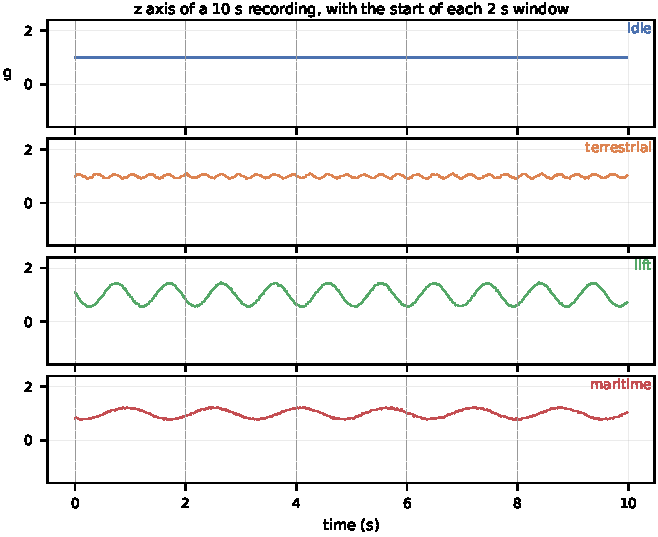
\includegraphics[width=\textwidth]{images/modules/MC-3/mc3_windows.pdf}
    \end{column}
    \begin{column}{0.44\textwidth}
      \small
      \begin{itemize}
        \item A window of 2 s, a new window every 0.2 s. Each window is one
              row of the dataset.
        \item The window must hold a few cycles of the motion. A window
              shorter than one cycle hides the frequency.
        \item The task of the lab is the transport of a container. It rests in
              a warehouse (\texttt{idle}), rides a truck or a train
              (\texttt{terrestrial}), is moved by a forklift
              (\texttt{lift}), or sails (\texttt{maritime}).
      \end{itemize}
    \end{column}
  \end{columns}
  \vskip 0.2em
\end{frame}

% --------------------------------------------------- 3. what a window hides
\begin{frame}{What the window hides}
  \begingroup\centering
  \begin{tikzpicture}[font=\scriptsize, >=stealth,
      st/.style={draw=coolgray, rounded corners=2pt, fill=boxgray,
                 align=center, text width=1.7cm, minimum height=1.3cm}]
    \node[st] (w) at (0,0) {2 s of\\ acceleration};
    \node[st] (s) at (3.4,0) {the power at\\ each frequency};
    \draw[->] (w) -- node[above, font=\scriptsize] {FFT} (s);
    \node[st, fill=cardinalred!12, minimum height=0.9cm] (n) at (7.4,0)
      {the position of\\ each oscillation\\ is not in the values};
    \draw[->] (s) -- (n);
  \end{tikzpicture}\par\endgroup
  \vskip 0.5em
  \small
  \begin{itemize}
    \item The network sees the shape of the signal. It has no way to ask
          which frequency the shape contains.
    \item The RMS of a window says how big the motion is. It says nothing
          about how fast it is.
    \item Two motions with the same size and different speed give the same
          RMS and different spectra.
  \end{itemize}
\end{frame}

% --------------------------------------------------------- 4. remove the mean
\begin{frame}{Remove the mean first}
  \begin{itemize}
    \item The kit lies with the display up, so the z axis shows gravity. Its
          value is near $+1$ g whatever the motion is.
    \item A large constant shifts every feature and hides the small changes
          that carry the class.
    \item Subtract the mean of the window from each sample. Bin 0 of the FFT
          is then zero, and the answer can start at bin 1.
  \end{itemize}
  \vskip 0.4em
  \keypoint{The RMS before the removal of the mean and after it are two
    different numbers.}
\end{frame}

% ------------------------------------------------------------------ 5. the RMS
\begin{frame}{The root mean square}
  \begin{equation*}
    x_{\mathrm{RMS}} = \sqrt{\frac{1}{n}\sum_{i=1}^{n} x_i^2}
  \end{equation*}
  \small
  \begin{itemize}
    \item One value for the size of the motion. It has the unit of the
          signal, so it stays in g.
    \item It is the value of a constant direct current that would give the
          same power in a resistor.
    \item It is the cheapest feature of the block, and it is in every
          version of it.
  \end{itemize}
  \vskip 0.3em
  \small The formulas in this module use no correction for the sample size.
  Then a laptop and a board give the same number.
\end{frame}

% ------------------------------------------- 6. skewness and kurtosis
\begin{frame}{Skewness and kurtosis}
  \begin{columns}[T]
    \begin{column}{0.46\textwidth}
      \small
      \begin{itemize}
        \item Skewness measures the asymmetry of the distribution of the
              values of a window. It is below zero when the long tail is on
              the left.
        \item Kurtosis measures how heavy the tails are. A normal
              distribution has 0.
        \item A value far from 0 says that the motion is not a smooth
              oscillation. It is a shock or a knock.
      \end{itemize}
    \end{column}
    \begin{column}{0.50\textwidth}
      \small
      \setlength{\tabcolsep}{3pt}
      \begin{tabular}{@{}L{2.1cm}L{2.7cm}@{}}
        \toprule
        Signal & Skewness, kurtosis \\
        \midrule
        Smooth sine wave & near 0, near -2 \\
        One shock in the window & large, large \\
        Sensor noise & near 0, near 0 \\
        \bottomrule
      \end{tabular}
    \end{column}
  \end{columns}
  \vskip 0.3em
  \small The kurtosis of a sine wave is $-1.5$, and the sample of a normal
  distribution is near $-2$, because the module subtracts 3.
\end{frame}

% ---------------------------------------------- 7. the formula decides
\begin{frame}{The formula decides the number}
  \begin{itemize}
    \item Two definitions of the skewness exist: one with a correction for
          the sample size, and one with no correction.
    \item For the z axis of the window of the project of the chapter, the
          Studio reports $-0.0978$, $0.1735$, and $6.8629$. The same values
          with the correction are $-0.0990$, $0.1756$, and $6.9463$.
    \item The two differ by about one percent on the third axis. A model
          trained on the values of one definition and run on the values of
          the other one loses accuracy.
  \end{itemize}
  \vskip 0.4em
  \keypoint{Write the formula in the report. A number without a formula is
    not a feature.}
  \source{Values reported in "Machine Learning Systems", chapter "DSP
    Spectral Features", for the window of the project.}
\end{frame}

% --------------------------------------- 8. the time-domain feature list
\begin{frame}{The time-domain features of one axis}
  \footnotesize
  \begin{tabular}{@{}L{3.6cm}L{3.0cm}L{3.0cm}@{}}
    \toprule
    Feature & What it measures & Version \\
    \midrule
    RMS & the size of the motion & 1 and 2 \\
    Skewness & the asymmetry of the values & 2 \\
    Kurtosis & the weight of the tails & 2 \\
    \bottomrule
  \end{tabular}
  \vskip 0.5em
  \small
  \begin{itemize}
    \item Three values per axis. The first version of the block computed
          only the RMS, plus the peaks and the power of the FFT, for 11
          values per axis and 33 values in total.
    \item The second version adds the skewness and the kurtosis, and the
          studio then reports 39 values, so 13 per axis.
  \end{itemize}
  \source{Feature lists of "Machine Learning Systems", chapter "DSP
    Spectral Features", versions 1 and 2 of the Spectral Analysis block.}
\end{frame}

% ---------------------------------------------------------------- 9. the FFT
\begin{frame}{The FFT turns samples into bins}
  \begin{equation*}
    \text{distance between two bins} = \frac{f_s}{N}
    \qquad
    \text{resolution} \approx \frac{1}{T}
  \end{equation*}
  \small
  \begin{itemize}
    \item $f_s$ is the sampling rate, $N$ is the FFT length, and $T$ is the
          length of the window.
    \item A window of 2 s at 50 Hz has 100 samples. An FFT of length 128
          pads it with 28 zeros. The bins then sit every $50/128 = 0.39$
          Hz, and no bin is closer than the $0.5$ Hz that 2 s of signal
          can resolve.
    \item Padding adds no information. It only draws the same peak on a
          finer grid.
  \end{itemize}
  \vskip 0.3em
  \keypoint{More bins means a finer grid, not a better sensor.}
\end{frame}

% ------------------------------------------------------- 10. the spectrum
\begin{frame}{The power at each frequency}
  \begingroup\centering
  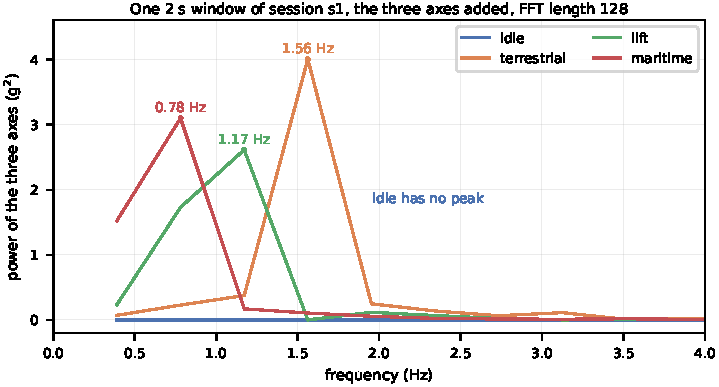
\includegraphics[width=0.95\textwidth]{images/modules/MC-3/mc3_power.pdf}
  \par\endgroup
  \vskip 0.2em
  \small Each class that moves has a band of its own, and \texttt{idle} has
  no band because it does not move. The rate of a class follows the speed of
  its session, so two bands can touch. The network sees 64 numbers per axis
  and no shape at all.
  \source{Figure drawn from the simulated signals of the lab notebook, with
    the power of the three axes added. The notebook plots one axis at a time.
    The signals are simulated, so the figure is an illustration.}
\end{frame}

% ------------------------------------------- 11. max-hold and Welch
\begin{frame}{Max-hold and Welch's method}
  \small
  \begin{itemize}
    \item A window has more samples than the FFT length. So the window is cut
          into frames, and the FFT runs on each frame.
    \item Welch's method averages the power of the frames. The estimate is
          smooth, and a peak that lasts a short time is reduced.
    \item The block of the studio keeps the largest power of each bin over
          all the frames. The function in the chapter divides the signal
          into frames, takes the power of each frame, and keeps the maximum.
    \item Max-hold keeps a short event. Welch removes it. Choose with the
          motion in mind: a pallet that hits once in a window is an event.
  \end{itemize}
  \source{Description and function of "Machine Learning Systems", chapter
    "DSP Spectral Features", section "Spectral features".}
\end{frame}

% ------------------------------------------ 12. the feature vector
\begin{frame}{The feature vector of one axis}
  \footnotesize
  \begin{tabular}{@{}L{3.6cm}L{2.2cm}L{2.6cm}@{}}
    \toprule
    Group & Values & FFT length \\
    \midrule
    RMS, skewness, kurtosis & 3 & any \\
    Spectral power of bins 1 to $N/2$ & $N/2$ & 128 \\
    \midrule
    One axis & 67 & 128 \\
    Three axes & 201 & 128 \\
    \bottomrule
  \end{tabular}
  \vskip 0.5em
  \small
  \begin{itemize}
    \item The block of the studio also gives the skewness and the kurtosis
          of the 16 power values. Add two values per axis when you need
          them.
    \item With no filter, the number of power values is half the FFT length.
  \end{itemize}
  \vskip 0.2em
  \source{Values of the example of this module. The rule "half the FFT
    length" is from "Machine Learning Systems", chapter "DSP Spectral
    Features".}
\end{frame}

% ------------------------------------------------- 13. the FFT length
\begin{frame}{The choice of the FFT length}
  \footnotesize
  \setlength{\tabcolsep}{4pt}
  \begin{tabular}{@{}L{2.3cm}L{2.3cm}L{2.4cm}L{2.3cm}@{}}
    \toprule
    FFT length & Bins, distance & Values, 3 axes & Parameters \\
    \midrule
    32 & 16, 1.56 Hz & 57 & 1414 \\
    64 & 32, 0.78 Hz & 105 & 2374 \\
    128 & 64, 0.39 Hz & 201 & 4294 \\
    \bottomrule
  \end{tabular}
  \vskip 0.5em
  \small
  \begin{itemize}
    \item The columns are one network with 20, 10, and 4 units, trained on
          the fallback dataset of the lab.
    \item Choose the length from the lowest frequency that separates two
          classes. Then check that the extra values still pay for
          themselves.
  \end{itemize}
  \source{Example model of this module, measured by the notebook of the
    lab on an x86 processor with AVX2. The values say nothing about a
    board.}
\end{frame}

% ------------------------------------------------------ 14. the wavelets
\begin{frame}{Wavelets: time and frequency together}
  \begin{columns}[T]
    \begin{column}{0.48\textwidth}
      \small
      \begin{itemize}
        \item The FFT of a window gives one spectrum for the whole window. A
              shock in the first half and a shock in the second half give
              the same spectrum.
        \item The wavelet transform cuts the signal into a low part and a
              high part. Repeating the cut gives more levels.
        \item Each level is a signal of its own, and the same features
              apply to it.
      \end{itemize}
    \end{column}
    \begin{column}{0.48\textwidth}
      \small
      \setlength{\tabcolsep}{3pt}
      \begin{tabular}{@{}L{3.2cm}L{1.1cm}@{}}
        \toprule
        Feature group & Values \\
        \midrule
        Statistics: n5, n25, n75, n95, median, mean, std, var, rms,
          skewness, kurtosis & 11 \\
        Zero crossing rate and mean crossing rate & 2 \\
        Entropy & 1 \\
        \midrule
        One level & 14 \\
        \bottomrule
      \end{tabular}
    \end{column}
  \end{columns}
  \vskip 0.2em
  \small With one level and no filter, 14 values for the signal and 14 for
  the low part, so 28 per axis and 84 for the three axes.
  \source{"Machine Learning Systems", chapter "DSP Spectral Features",
    section "Wavelets".}
\end{frame}

% ------------------------------------------------------- 15. the measurement
\begin{frame}{What the module measures}
  \begingroup\centering
  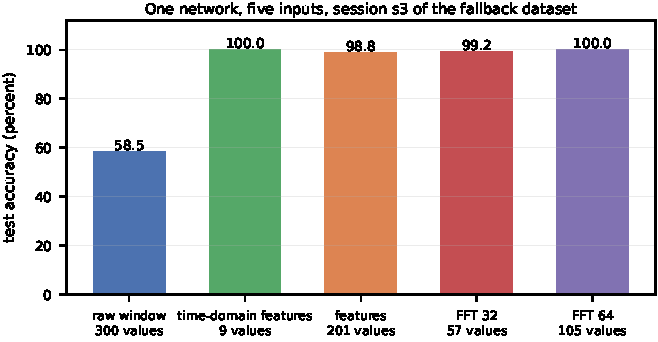
\includegraphics[width=0.88\textwidth]{images/modules/MC-3/mc3_inputs.pdf}
  \par\endgroup
  \vskip 0.2em
  \small The network on the raw window fails on this dataset: 1312 training
  windows are too few for 300 inputs. The nine time-domain values are
  enough. The 192 power values add nothing here.
  \source{One run of the lab notebook on the fallback dataset of the module,
    an x86 processor with AVX2. The signals are simulated.}
\end{frame}

% ------------------------------------------------------ 16. what to remember
\begin{frame}{What to remember}
  \small
  \begin{enumerate}
    \item A window of 2 s at 50 Hz gives 100 samples per axis. Cut the
          recording with a stride, so the windows overlap.
    \item Remove the mean first. Then compute the RMS, the skewness, and
          the kurtosis, and write the formula.
    \item The FFT length sets the number of bins and the distance between
          two bins. Padding adds no information.
    \item Keep the largest power of each bin over the frames when the
          motion has short events.
    \item The feature set is a trade-off. Measure the accuracy and the
          model size before you choose it.
  \end{enumerate}
\end{frame}

% ------------------------------------------------------------- exercise
\exerciseframe{Bins down to 0.4 Hz}{
  A window of 2 s is recorded at 50 Hz. You need the power at every
  frequency down to 0.4 Hz, and you want the fewest values that still reach
  that frequency.

  \begin{enumerate}
    \item Give the FFT length.
    \item Give the number of values of one axis, with the three
          time-domain features.
    \item Give the number of values of the vector of the three axes.
  \end{enumerate}
}

\answerframe{Bins down to 0.4 Hz}{
  \begin{enumerate}
    \item The distance between two bins is $f_s / N$, so $50 / N \leq 0.4$
          gives $N \geq 125$. The next power of two is $N = 128$. A window
          of 2 s cannot resolve less than $0.5$ Hz, so 128 bins are enough
          for the grid and the data.
    \item Bin 0 carries the mean, which is zero after the removal, so the
          answer starts at bin 1. The power values are $128/2 = 64$, and
          with the three time-domain features one axis has $3 + 64 = 67$
          values.
    \item The three axes have $3 \times 67 = 201$ values. A network with 20,
          10, and 4 units then has 4294 parameters.
  \end{enumerate}
  \vskip 0.3em
  \small The answer of part 1 is the smallest FFT length that reaches
  0.4 Hz. Whether 201 values are worth their place is a question of
  measurement, not of arithmetic: the lab measures it.
}
% A module of type T+L keeps the lab part. A module of type T deletes the
% next line and the file lab.tex.
% Lab part of the module.
%
% Module MC-3 of Section 6.1 of the syllabus: "Spectral features for motion
% data". Type T+L, 90 minutes: about 45 minutes of theory and 45 minutes of
% lab. The lab needs no board. It runs on the recordings of a group, or on
% the simulated fallback dataset of its folder.
%
% The parts follow the README of the lab folder. The frame of the expected
% output shows the form of the output and the values that check the method.
% No value here is a measurement of a board.

% --------------------------------------------------------------- 1. the goal
\begin{frame}{Lab: goal and plan}
  \small
  \begin{itemize}
    \item \textbf{Goal.} You compute the features of a motion signal, train
          a small classifier on them, and compare five inputs for the same
          task.
    \item \textbf{Deliverable.} The table of section 8 of the notebook,
          copied into \code{report.md}, and the answers of its three questions.
  \end{itemize}
  \vskip 0.5em
  \footnotesize
  \setlength{\tabcolsep}{4pt}
  \begin{tabular}{@{}L{1.0cm}L{7.2cm}L{1.5cm}@{}}
    \toprule
    Part & Content & Time \\
    \midrule
    A & The data, the windows, and the three time-domain features & 12 min \\
    B & The FFT and the spectral power of one axis & 13 min \\
    C & The classifier, and its number of parameters & 8 min \\
    D & Five inputs for the same task, and the FFT length & 12 min \\
    \bottomrule
  \end{tabular}
  \vskip 0.5em
\end{frame}

% ------------------------------------------------------------ 2. the files
\begin{frame}{Lab: files and data}
  \small
  \setlength{\tabcolsep}{4pt}
  \begin{tabular}{@{}L{3.9cm}L{5.3cm}@{}}
    \toprule
    File & Content \\
    \midrule
    \code{spectral\_features.ipynb} & The notebook. It has four tasks. \\
    \code{host/motion\_sim.py} & The simulated signals. \\
    \code{host/make\_dataset.py} & Makes the fallback dataset. \\
    \code{report.md} & The report to hand in. \\
    \code{solutions/} & The notebook with all tasks complete and with its output, and an example report. \\
    \bottomrule
  \end{tabular}
  \vskip 0.5em
  \small
  \begin{itemize}
    \item The notebook reads the folder \code{data/} when it has recordings of
          the format of the course. Otherwise it makes the simulated
          dataset in \code{fallback\_data/}.
    \item The last session is the test session. A model that separates the
          sessions has learned the person, not the motion.
  \end{itemize}
\end{frame}

% ---------------------------------------------------------------- 3. part A
\begin{frame}[fragile]{Part A: the data and the time features (12 min)}
  \small
  \begin{enumerate}
    \item Start Jupyter from the folder of the lab:
\begin{lstlisting}[style=shell]
../../../.venv/bin/jupyter lab spectral_features.ipynb
\end{lstlisting}
    \item Run section 1. Write the number of training windows and of test
          windows in the report.
    \item \textbf{Task 1.} Write \code{time\_features(window)}: the RMS, the
          skewness, and the kurtosis of one axis, after the removal of the
          mean.
    \item Run the cell after the task.
  \end{enumerate}
  \vskip 0.5em
  \small You see the check of the task, and the three values for the first
  window:
  \begin{center}
  \begin{tabular}{@{}lll@{}}
    \toprule
    RMS & Skewness & Kurtosis \\
    \midrule
    0.0038 & $-0.3266$ & $-0.0771$ \\
    \bottomrule
  \end{tabular}
  \end{center}
  \small The first window is an idle window, so its values are small. That
  is the answer of the check, not a target for your own window.
  \source{Values of one run of the solution notebook on the fallback
    dataset, an x86 processor with AVX2.}
\end{frame}

% ---------------------------------------------------------------- 4. part B
\begin{frame}{Part B: the FFT and the spectral power (13 min)}
  \small
  \begin{enumerate}
    \item Run section 3. The cell draws the spectral power of one window of
          each class on the z axis. The z axis of \code{terrestrial} is almost
          still, because the motion of a truck sits in the horizontal plane.
          Write in the report which frequency holds the power of the class
          \code{lift}, and which one holds the power of \code{maritime}.
    \item \textbf{Task 2.} Write \code{axis\_features(window, nfft)}: the three
          time-domain features, then the power of bins 1 to \code{nfft // 2}.
    \item Run the cell after the task, then section 4.
  \end{enumerate}
  \vskip 0.5em
  \small You see the number of values of one axis, and it must be
  $3 + 128 / 2 = 67$. Then the feature matrix has 201 columns and the
  notebook prints the mean and the standard deviation of the first nine
  features.
  \vskip 0.3em
\small The first three values of the feature vector are the RMS, the
skewness, and the kurtosis of the axis `x`. The next six are power values.
\end{frame}

% ---------------------------------------------------------------- 5. part C
\begin{frame}{Part C: the classifier (8 min)}
  \small
  \begin{enumerate}
    \item \textbf{Task 3.} Write \code{make\_model(n\_inputs)}: a layer of 20 units
          with ReLU, a layer of 10 units with ReLU, and 4 outputs with
          softmax.
    \item Run the cell after the task. The check calculates the expected
          number of parameters itself.
    \item Run the next cell to train it.
  \end{enumerate}
  \vskip 0.5em
  \begin{center}
  \begin{tabular}{@{}l@{}}
    \toprule
    input values 201, parameters 4294 (expected 4294), outputs 4 \\
    the model on the spectral features: 4294 parameters, \\
    test accuracy 98.8 percent \\
    \bottomrule
  \end{tabular}
  \end{center}
  \small The names of the layers and of the input matter. Without them, the
  file of the model changes size with each model that the notebook builds.
  \source{Values of one run of the solution notebook on the fallback
    dataset, an x86 processor with AVX2.}
\end{frame}

% ---------------------------------------------------------------- 6. part D
\begin{frame}{Part D: five inputs for the same task (12 min)}
  \small
  \begin{enumerate}
    \item Run section 6. It trains the same network on the raw window, on
          the time-domain features, and on the spectral features.
    \item Write the three lines of output in the report.
    \item \textbf{Task 4.} Before you run section 7, complete the table with
          the number of values of one axis for the FFT lengths 32, 64, and
          128. Then write the length that you expect to win, and why.
    \item Run section 7 and section 8, and copy the table into the report.
  \end{enumerate}
  \vskip 0.4em
  \small The notebook prints the same table as the figure of the lecture:
  the raw window reaches 58.5 percent, the nine time-domain values reach
  100.0 percent, and the spectral values reach 98.8 percent with an FFT
  length of 128.
  \source{Values of one run of the solution notebook on the fallback
    dataset, an x86 processor with AVX2. The signals are simulated.}
\end{frame}

% ------------------------------------------------------------ 7. the check
\begin{frame}{Check criterion and Decision Log}
  \small
  \begin{itemize}
    \item The notebook prints \code{complete} for tasks 1, 2, 3, and 4.
    \item The table of the report has five rows, each with the number of
          values, the number of parameters, and a measured test accuracy.
    \item The three questions of the report have answers with numbers from
          your own run.
    \item The Decision Log names one decision and one number.
  \end{itemize}
  \vskip 0.5em
  \keypoint{Question of the Decision Log: a device must classify the motion
    of a pallet for a year on a battery. Which feature set do you put in
    the firmware, and which number of your table decides it?}
\end{frame}

% ------------------------------------------------------- 8. common problems
\begin{frame}{Common problems}
  \small
  \begin{tabular}{@{}L{4.4cm}L{5.0cm}@{}}
    \toprule
    Problem & Fix \\
    \midrule
    The notebook says that it uses the fallback dataset & Your group has no
      recording in \code{data/}. The signals are simulated. \\
    \code{Task 2} says that the answer needs 67 values & Your answer has a
      different number. Return one value for each bin. \\
    \code{Task 3} says that the model raises an error & A layer is missing, or a
      layer is added with a tensor instead of with its input. \\
    The accuracies change between two runs & Write the seed, and run the
      same cells again. \\
    \bottomrule
  \end{tabular}
  \vskip 0.5em
  \small The README of the lab folder has the full list of the checks of the
  notebook and the run time.
\end{frame}
% Credits frame. Section 10 of the syllabus gives this text.
% Each deck ends with this frame:
%   % Credits frame. Section 10 of the syllabus gives this text.
% Each deck ends with this frame:
%   % Credits frame. Section 10 of the syllabus gives this text.
% Each deck ends with this frame:
%   \input{sections/credits}
%
% The list \coursecredits selects the sources. preamble/course.tex gives the
% default list and one command for each source. The main file of a deck
% changes the list before it inputs this file, so that the frame names only
% the sources that the deck uses:
%   \renewcommand{\coursecredits}{\creditmlsys\creditxiao}
\begin{frame}[allowframebreaks]{Credits}
  \vskip 0.6em
  \begin{itemize}\footnotesize\itemsep 0.4em
    \coursecredits
  \end{itemize}
  \vskip 0.8em
\end{frame}

%
% The list \coursecredits selects the sources. preamble/course.tex gives the
% default list and one command for each source. The main file of a deck
% changes the list before it inputs this file, so that the frame names only
% the sources that the deck uses:
%   \renewcommand{\coursecredits}{\creditmlsys\creditxiao}
\begin{frame}[allowframebreaks]{Credits}
  \vskip 0.6em
  \begin{itemize}\footnotesize\itemsep 0.4em
    \coursecredits
  \end{itemize}
  \vskip 0.8em
\end{frame}

%
% The list \coursecredits selects the sources. preamble/course.tex gives the
% default list and one command for each source. The main file of a deck
% changes the list before it inputs this file, so that the frame names only
% the sources that the deck uses:
%   \renewcommand{\coursecredits}{\creditmlsys\creditxiao}
\begin{frame}[allowframebreaks]{Credits}
  \vskip 0.6em
  \begin{itemize}\footnotesize\itemsep 0.4em
    \coursecredits
  \end{itemize}
  \vskip 0.8em
\end{frame}


\end{document}